\section{Creating transistor structures}
Unfortunately I did not manage to complete this task since it took me much longer than expected to undcerstand the lsVienna framework.
Therefore I will present only the steps that I did manage to complete and discuss possible further outcomes.

\subsection{Processing steps}
All axis units are in nanometers

\begin{figure}[H]
	\centering
	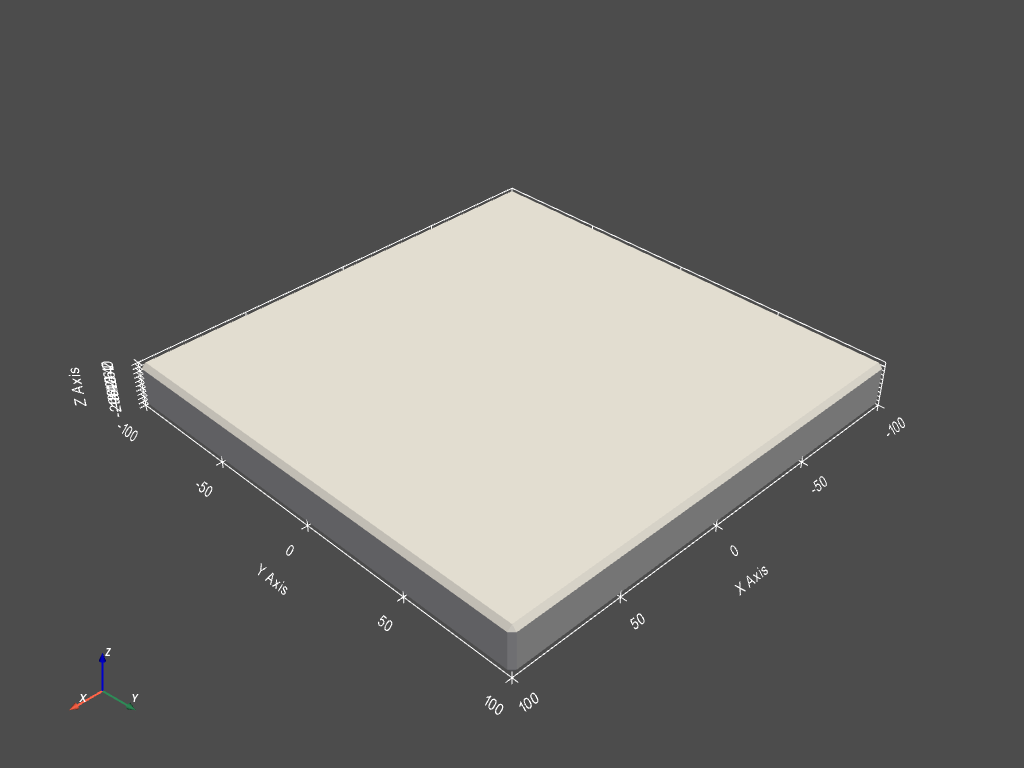
\includegraphics[width=0.75\textwidth]{res/task3_1_oxide_deposition.png}
	\caption{Step 1: Starting with a single 200x200x20nm plate of silicon}
\end{figure}

\begin{figure}[H]
	\centering
	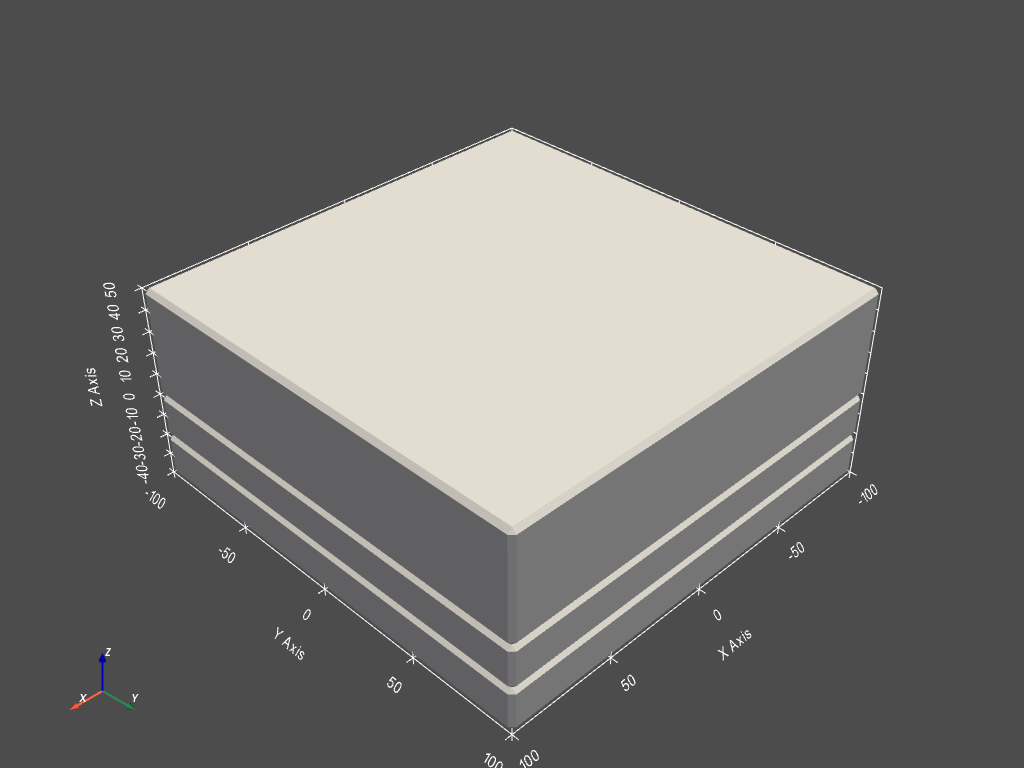
\includegraphics[width=0.75\textwidth]{res/task3_2_silicon_deposition.png}
	\caption{Step 2: Depositing Oxide (middle) and mask (top) on the silicon substrate}
\end{figure}

\begin{figure}[H]
	\centering
	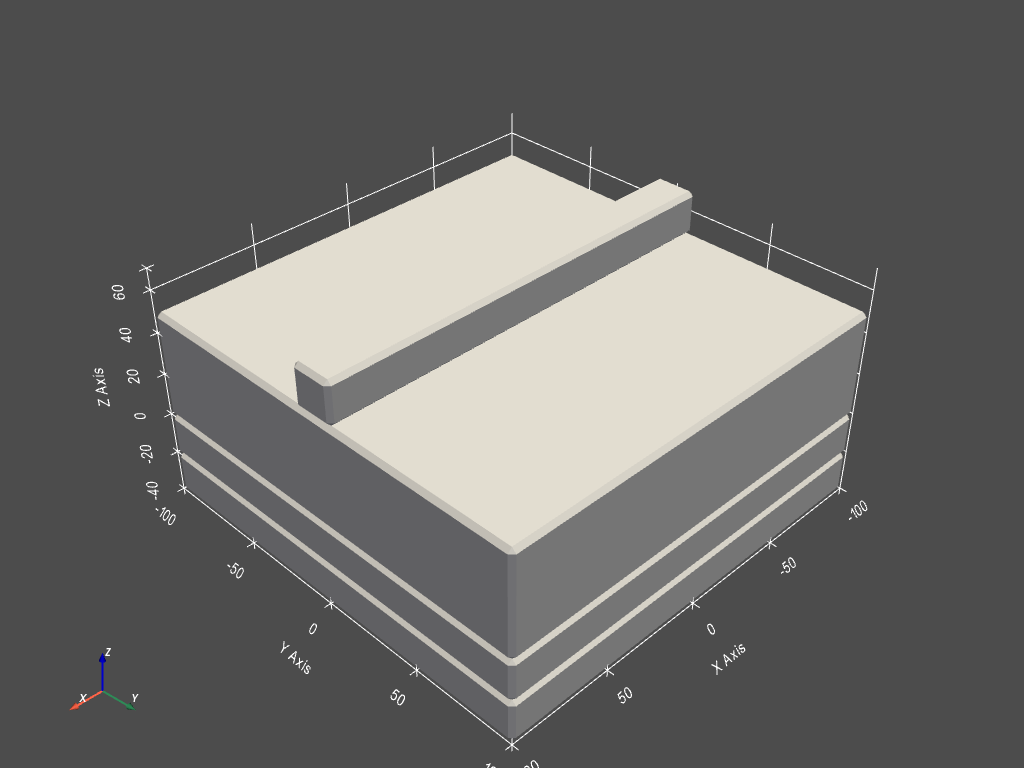
\includegraphics[width=0.75\textwidth]{res/task3_3_mask_cration.png}
	\caption{Step 3: Creating a mask on top of the silicon}
\end{figure}

\begin{figure}[H]
	\centering
	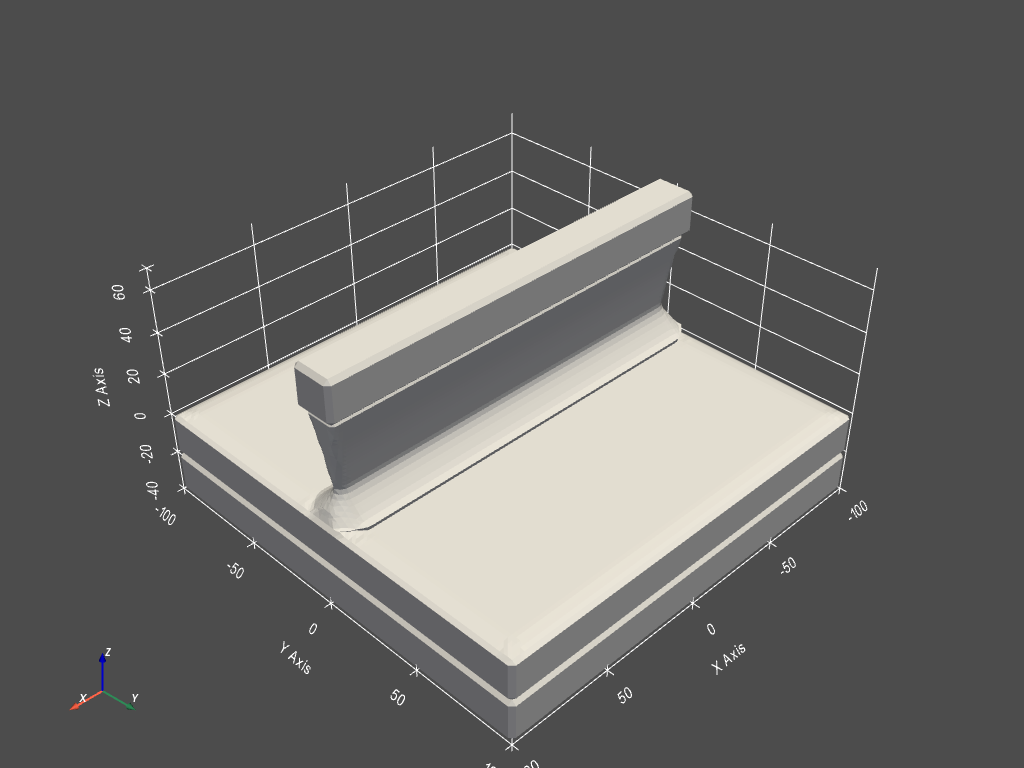
\includegraphics[width=0.75\textwidth]{res/task3_4_fin_creation.png}
	\caption{Step 4: Directionally etching downwards. Etching is not perfectly vertical but is slightly "digging" below the mask.}
    \label{ffig:fin-creation}
\end{figure}

\begin{figure}[H]
	\centering
	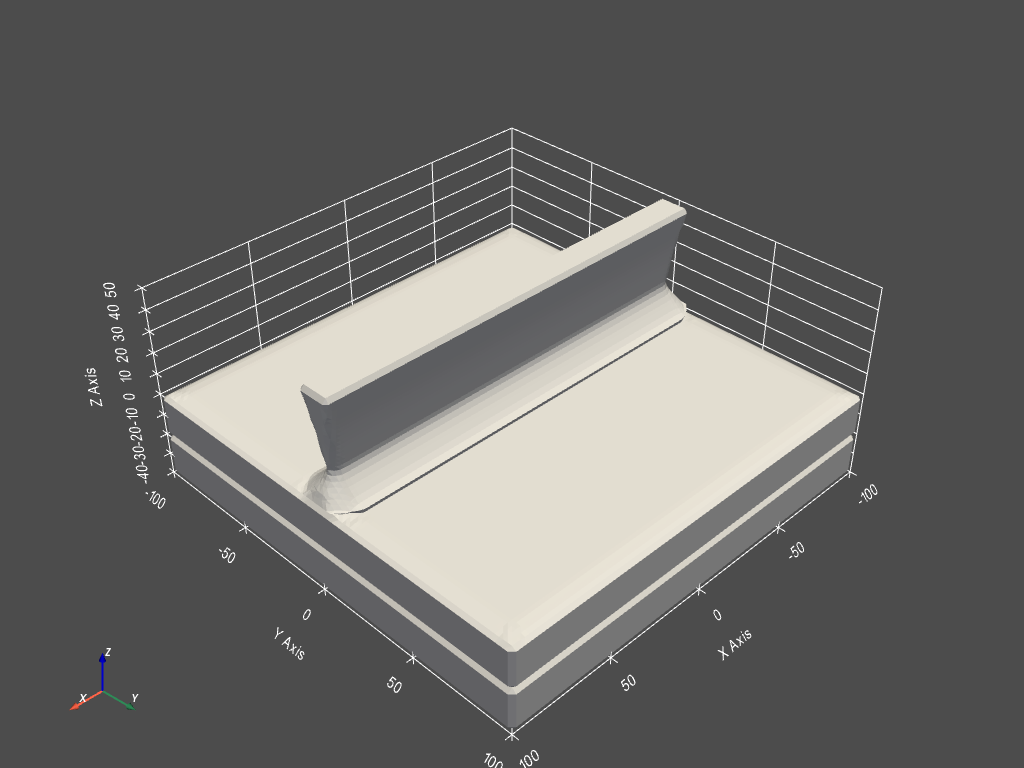
\includegraphics[width=0.75\textwidth]{res/task3_5_maskRemoval.png}
	\caption{Step 5: Mask removal}
\end{figure}


\begin{figure}[H]
	\centering
	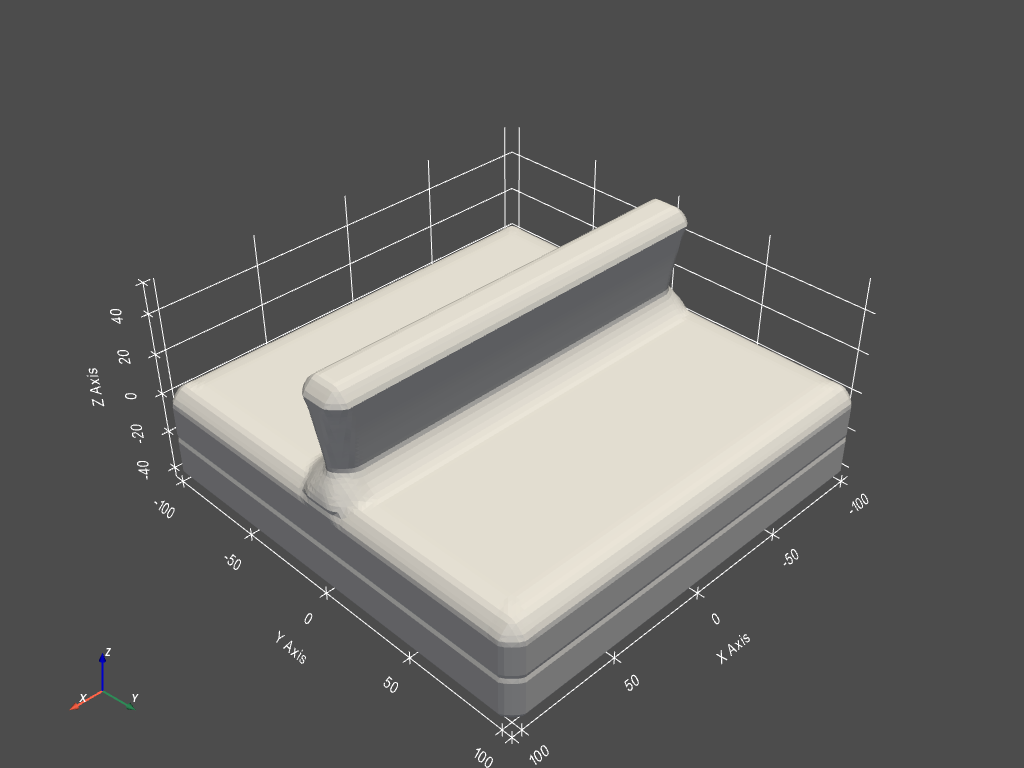
\includegraphics[width=0.75\textwidth]{res/task3_6_spacerDeposition.png}
	\caption{Step 6: Uniform spacer deposition}
    \label{fig:spacer-deposition}
\end{figure}


\begin{figure}[H]
	\centering
	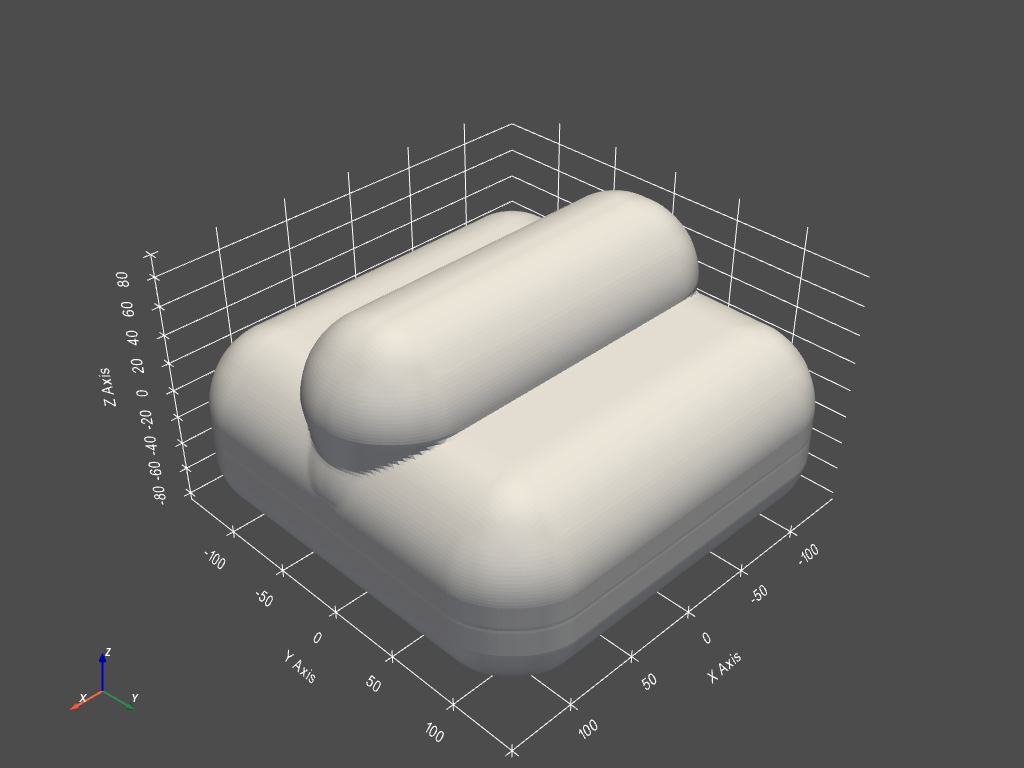
\includegraphics[width=0.75\textwidth]{res/task3_7_gateDeposition.png}
	\caption{Step 7: Gate deposition}
    \label{fig:gate-deposition}
\end{figure}

One can see that something is not working in step 7 (Fig. \ref{fig:gate-deposition}).
I suspect that the reason behind this is the absence of properly defined boundary conditions or I am not defining materials correctly.
Unfortunately at this step I have run out of time to fix issues.

However if that problem would be fixed creating the gate structure should be analog to creating the fin structure.

As seen in \ref{ffig:fin-creation} the etching process is not perfectly straigh but a slight anisotropy is rpesent.
This results in a smaller cross section near the base of the fin. If we would continue to etch then the fin would just break off.

If a positive isotropic component where to be introduced than etched structures would have walls that are skewed outwards instead of inwards (as shown in Fig. \ref{ffig:fin-creation}).





